\chapter{Second Task}
    \section{Presence of distractors}
        To discriminate between rods and distractors, I filtered blobs based on their area.
        In particular, I computed a reasonable confidence interval for this statistic based on the images of the first task (from 1280 to 6000).

        I considered Haralick's circularity and Hu's moments as possible alternatives but eventually decided to go for the area as it was easier to construct a confidence interval 
        without having to use discriminative algorithms as isolation forests to separate the two classes.

    \section{Partially overlapping rods}
        As a first attempt, I tried to separate touching rods by applying morphological operators and the Watershed segmentation algorithm.

        Unfortunately, due to the particular shape of the rods, I was not able to correctly tell apart the different rods.
        
        Therefore I decided to opt for a more complex approach, involving the identification of points of discontinuity in the shape of the rods, 
        to eventually draw the smallest possible line to reconstruct the original boundaries.
        
        Since by definition convexity defects are the deepest points between convex hulls where convexity is violated, 
        the points of contact between the rods will always be among them.
        
        Clearly, these two points are not the only convexity defects in the image, therefore they must be somehow identified 
        among all the others.
                
        Given the particular smooth shape of the rods, by performing Harris corner detection on the image, we can easily tell apart 
        the cluster of corner points around the points of contact between the rods.
        
        This way, after having found the center of these clusters, the exact points of contact can be described as the pairs of convexity 
        defect points closest to the centers of the clusters.

        This can be visually understood by looking at \ref{fig:cvx_defects}.

        \vspace{5 mm}
        \begin{figure}[h]
            \centering
            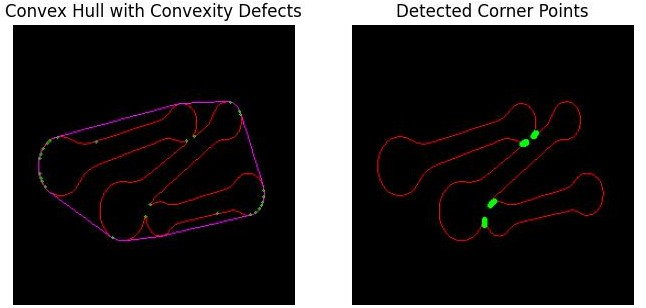
\includegraphics[scale=0.7]{cvx_defects.jpg}
            \caption{Convex hull with convexity defects highlighted and points detected by Harris corner detection algorithm.}
            \label{fig:cvx_defects}
        \end{figure}

    \section{Presence of iron powder over the inspection area}
        
        While on one hand the iron powder could be handled as if it was salt and pepper noise, through application of a median filter, on the other hand, the distribution of 
        the pixels' intensity of the dust particles closely resemble that of the rods' pixels, making it difficult to filter them when in close contact with the rods.

        In addition, repeated application of a median filter, even with a small kernel size (equal to $3$) would result in a degradation of the contours of the rods in those areas 
        where the they are particularly thin (e.g. around the holes).

        For these reasons I decided to test two different methodologies: applying a bilateral gaussian filter, and sharpening the image after the repeat application 
        of a median filter.

        Since the first approach failed at removing most of the dust particles from the image (leaving this task to the filtering stage over the connected components), I eventually 
        decided to opt for the second approach.

        In particular, the sharpened version of the image is obtained by adding to the image the difference between the image itself and its smoothed version (through application 
        of gaussian filtering).